\section{What Is Simulation?}

Astronomy is an observation science.
Unlike in terrestrial physics, we do not have the luxury of being able
to build a model system and do physical experimentation on it to understand
the core physics.  We have to take what nature gives us.
Simulation enables us to build a virtual model of a system and allows us
to do virtual experiments to understand how this system reacts to a range
of conditions and assumptions.  

It's tempting to think that one can download a simulation code, set a
few parameters, maybe edit some initial conditions, run, and then have
a virtual realization of some astrophysical system that you are
interested in.  Just like that.  In reality, it does not work that
way.  All simulation codes make approximations.  These start even
before one turns to the computer, simply by making a choice of what
equations are to be solved.  Typically, we have a system of PDEs,
and we need to convert the continuous functional form of our system
into a discrete form that can be represented in the finite memory of 
a computer.  This introduces yet more approximation.  V\&V

Blindly trusting the numbers that come out of the code is a recipe
for disaster.  You don't stop being a physicist the moment you execute
the code---you job as a computational scientist is to make sure that
the code is producing reasonable results, by testing it against known
problems and your physical intuition.  

Simulations should be used to gain insight and provide a physical
understanding.  
Because the systems we solve are so nonlinear, small changes in the
code or the programming environment (compilers, optimization, etc.)
can produce large differences in the numbers coming out of the code.
That's not a reason to panic.
As such its best not to obsess about precise numbers, but rather the
trends.  To really understand the limits of your simulations, you
should do parameter and convergence studies.

There is no \"uber-code.  Every algorithm begins with approximations
and has limitations.  Comparisons between different codes are
important and common in our field.  It builds confidence in the
results that we are on the right track.

To really understand your simulations, you need to know what the code
your are using is doing under the hood.  This means understanding the 
core methods used in our field.  These notes are designed to provide
a basic tour of some of the more popular methods, referring to the 
key papers for full derivations and details.  A companion python code,
{\sf pyro} is available to help. 


\section{Numerical Basics}

We assume a familiarity with basic numerical methods, which we
summarize below.  Any book on numerical methods can provide a
deeper discussion of these methods.

\subsection{Sources of Error}

With any algorithm, there are two sources of error we are concerned
with: {\em roundoff error} and {\em truncation error}.  

Roundoff arises from the error inherent in representing a floating
point number with a finite number of bits in the computer memory.  An
excellent introduction to the details of how computers represent
numbers is provided in \cite{goldberg:1991}.  

\begin{exercise}[Machine epsilon]
To see roundoff error in action, write a program to find the value
of $\epsilon$ for which $1 + \epsilon = 1$.  This value of $\epsilon$
is called {\em machine epsilon}.  You will get a different value for
single- vs.\ double-precision floating point arithmetic.
\end{exercise}

Some reorganization of algorithms can help minimize roundoff,
e.g.\ avoiding the subtraction of two very large numbers by factoring as:
\begin{equation}
x^3 - y^3 = (x - y)(x^2 + xy + y^2)
\end{equation}
but roundoff error will always be present at some level.

Truncation error is a feature of an algorithm---we typically
approximate an operator or function by expanding about some small
quantity.  When we throw away higher-order terms, we are truncating
our expression, and introducing an error in the representation.  If
the quantity we expand about truely is small, then the error is small.
A simple example is to consider the Taylor series representation of
$\sin(x)$:
\begin{equation}
\sin(x) = \sum_{n=1}^\infty (-1)^{n-1} \frac{x^{2n-1}}{(2n-1)!} 
\end{equation}
For $|x| \ll 1$, we can approximate this as:
\begin{equation}
\sin(x) \approx x - \frac{x^3}{6}
\end{equation}
in this case, our truncation error has the leading term $\propto x^5$,
and we say that our approximation is $\mathcal{O}(x^5)$, or
$5^\mathrm{th}$-order accurate.

\begin{exercise}[Convergence and order-of-accuracy]
We will be concerned with the order-of-accuracy of our methods, and a
good way to test whether our method is behaving properly is to perform
a convergence test.  Consider our $5^\mathrm{th}$-order accurate
approximation to $\sin(x)$ above.  Pick a range of $x$'s ($< 1$), and
compute the error in our approximation as $\epsilon \equiv \sin(x) - [
  x - x^3/6 ]$, and show that as you cut $x$ in half, $\epsilon$
reduces by $2^5$---demonstrating $5^\mathrm{th}$-order accuracy.
\end{exercise}


\subsection{Root Finding}

The most popular method for root finding is the Newton-Raphson method.
This arises from a Taylor expansion.

\subsection{Differentiation and Integration}

For both of these processes, there are two cases we might encounter.
In the first, we have function values at a discrete number of points
and we want to compute the derivative at a point or integration over a
range of points.  The second case is when we know a function
analytically and we want to construct a derivative or integral of this
function numerically.  In these notes, we'll be concerned only with
the first case.

\subsection{ODEs}


\begin{figure}[t]
\centering
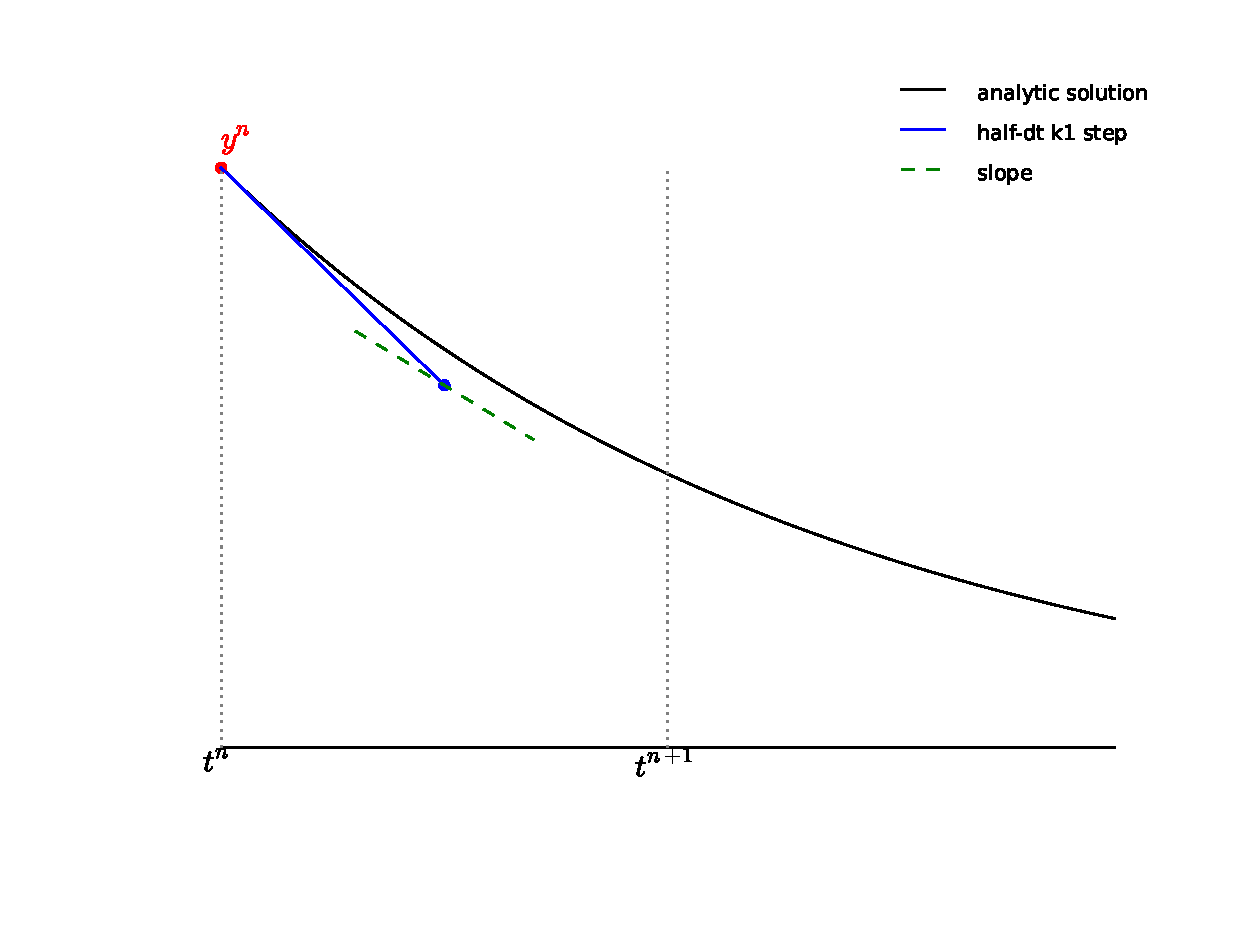
\includegraphics[width=3.2in]{rk4_k1.eps} 
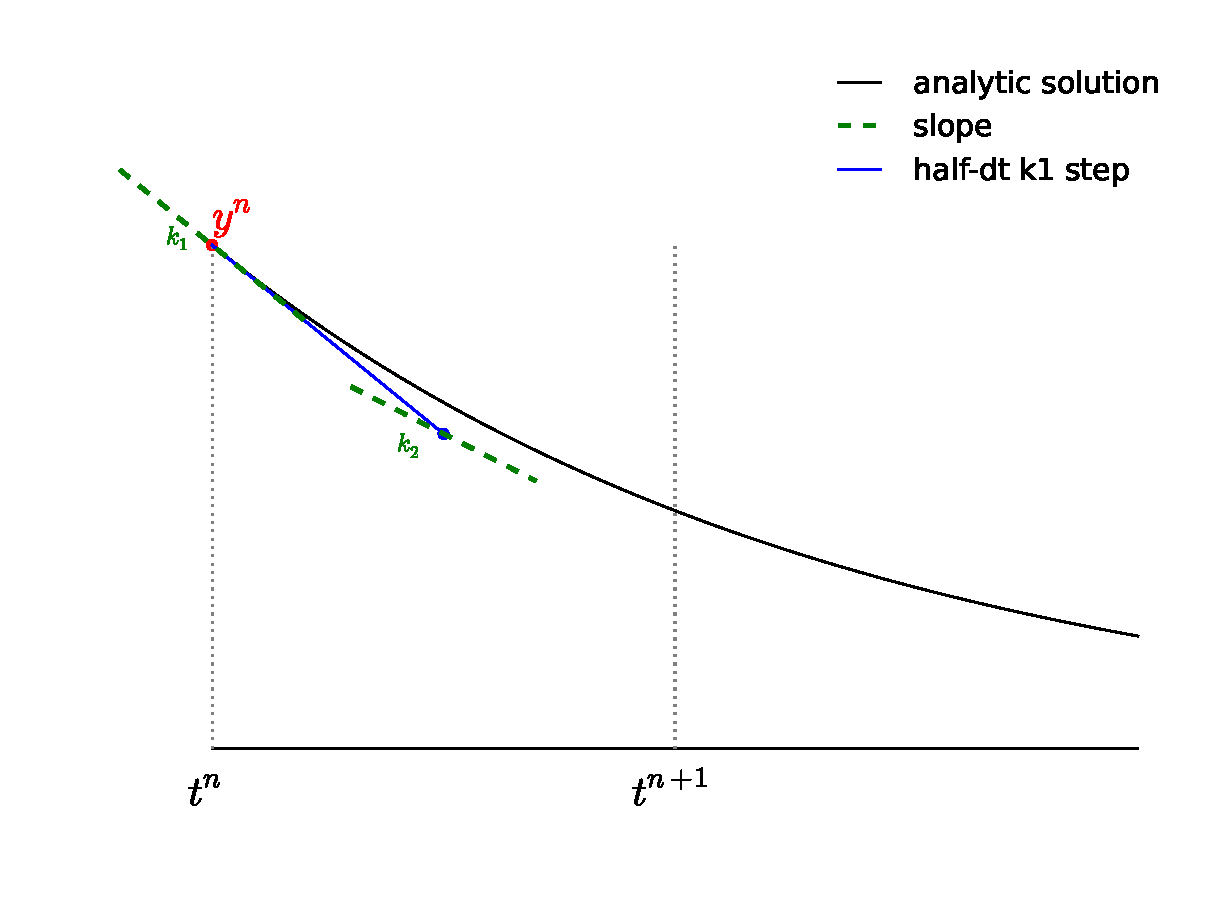
\includegraphics[width=3.2in]{rk4_k2} \\
%
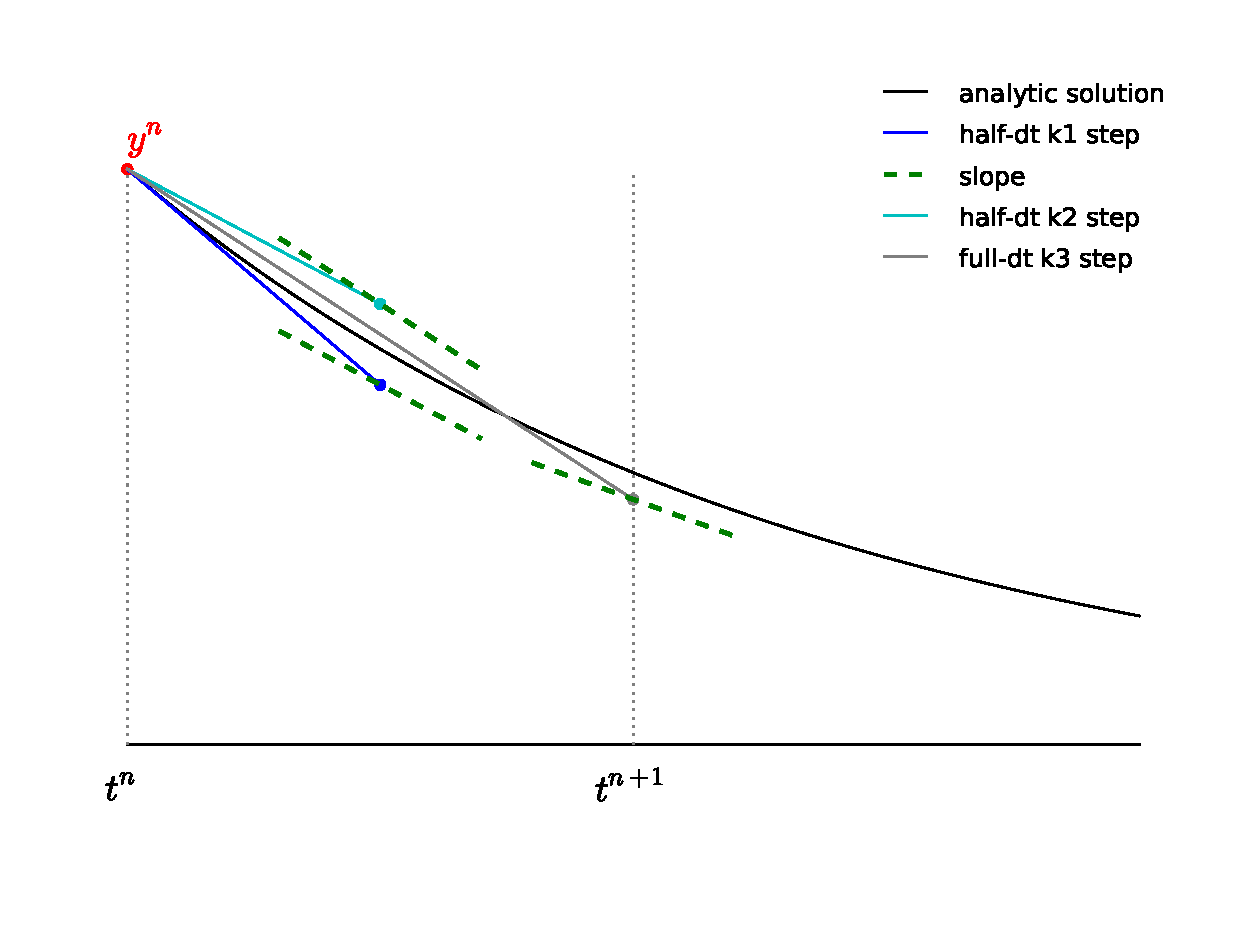
\includegraphics[width=3.2in]{rk4_k3.eps} 
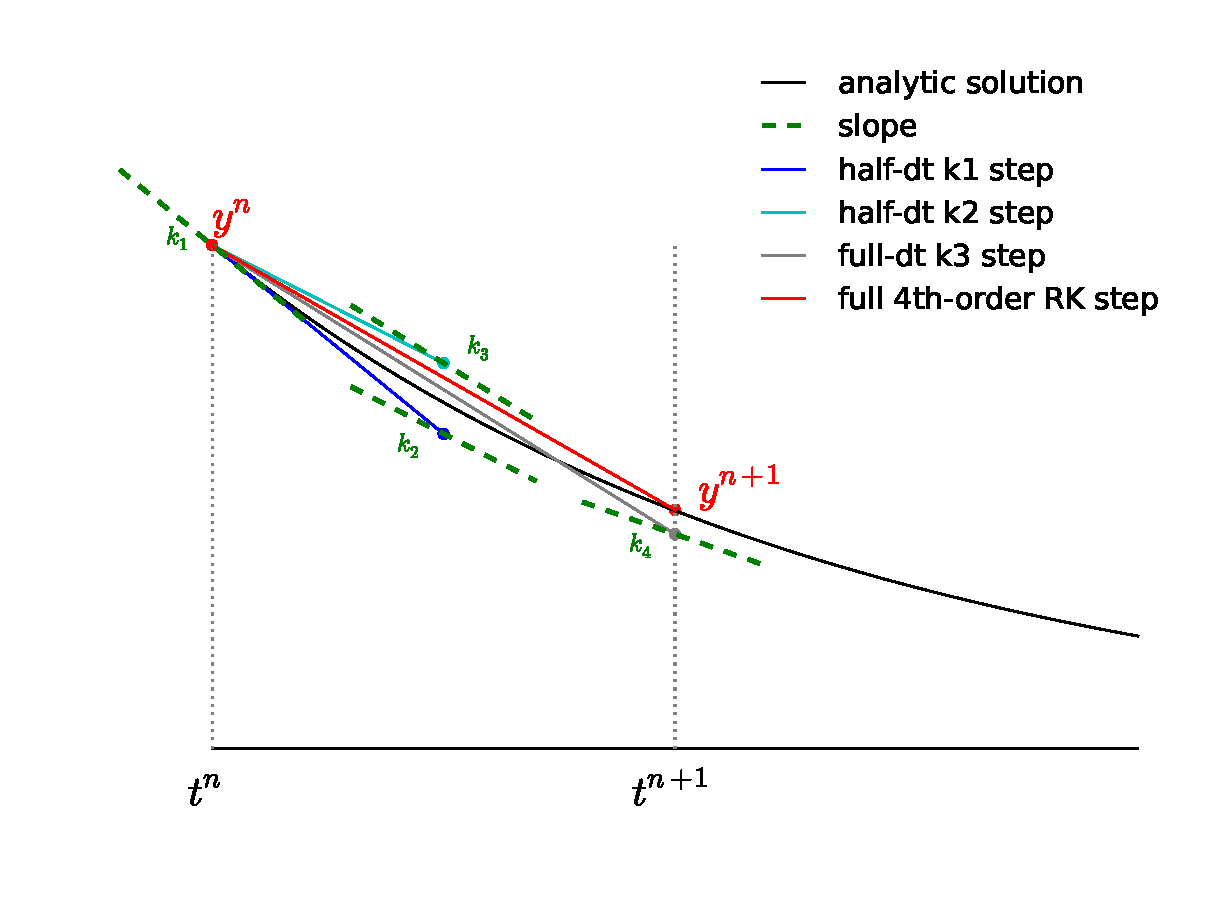
\includegraphics[width=3.2in]{rk4_final.eps} \\
%
\caption{\label{fig:rk} A graphical illustration of the $4^\mathrm{th}$-order
Runge-Kutta method.}
\end{figure}

\section{A Sample of Public Codes}

There are a large number of freely-available codes for modeling astrophysical
flows.
